% ------------------------------------------------------------------------------
% Este fichero es parte de la plantilla LaTeX para la realización de Proyectos
% Final de Grado, protegido bajo los términos de la licencia GFDL.
% Para más información, la licencia completa viene incluida en el
% fichero fdl-1.3.tex

% Copyright (C) 2012 SPI-FM. Universidad de Cádiz
% ------------------------------------------------------------------------------

En este capítulo detallaremos los diferentes tipos de pruebas que se han llevado a cabo para comprobar que la aplicación desarrollada funciona adecuadamente y de acuerdo con los requisitos previamente establecidos. 

\section{Pruebas unitarias}

En este tipo de pruebas se comprueba el correcto funcionamiento de un módulo de código. Se crearon pruebas unitarias, realizadas manualmente, para cada nueva funcionalidad del sistema, para más tarde integrar ese módulo en correcto funcionamiento en el sistema.

\section{Pruebas de integración}

Este tipo de pruebas tienen por objetivo localizar errores en subsistemas completos, analizando la interacción entre varios artefactos software. Se crearon pruebas manuales para cada subsistema, comparando que todas las pruebas unitarias funcionasen correctamente en conjunto.

\section{Pruebas de sistema}

En este tipo de pruebas se comprobaron que no existían discrepancias entre la aplicación realizada y sus objetivos o requisitos establecidos anteriormente.

\subsection{Pruebas funcionales}

Se realizaron pruebas para probar los flujos normales y alternativos de cada caso de uso:\\

Se comenzó a probar el sistema por la ventana de logueo. En ésta se comprobó que funcionase correctamente, es decir, que el usuario hiciera el login en la aplicación correctamente, que se respetaran las funcionalidades del sistema para cada tipo de usuario, que funcionara correctamente la protección de rutas y controladores. También se hicieron pruebas en la funcionalidad del sistema de pérdida de contraseña.\\

Se verificaron que los subsistemas dedicados a los clientes, proveedores, productos y familias funcionasen correctamente, es decir, se comprobaron los registros de cada uno de ellos introduciendo datos incorrectos para ver que el software indicase los errores, se comprobó la modificación de cualquier registro, así como la eliminación de cualquier registro teniendo especial cuidado en los casos que no se permitía eliminar (Ej: Borrar cliente cuando tiene operaciones).\\

Se comprobaron que las ventas, reservas, apartados y devoluciones funcionasen correctamente teniendo especial cuidado en los datos de entrada. Se verificó que los documentos generados fuesen correctos así como las operaciones almacenasen correctamente los datos.\\

En el subsistema de citas de comprobó la inserción, eliminación y modificación de una cita. En este subsistema se comprobó de manera detallada casos como no se podía crear una cita con un médico que está de vacaciones o con una baja. No se podía crear una cita con un cliente que ya tiene una cita en esa fecha.\\

En el subsistema de pedidos se comprobaron que se efectuaban los pedidos correctamente incluyendo los documentos generados así como la actualización correcta de los stocks de los productos cuando se recepcionaban.\\

En el subsistema de informes, se comprobó que sólo pudiesen generar los informes los médicos, y también se comprobaron que se mostraban los informes correctamente.\\

Se comprobó que el subsistema de gestión de empleados funcionaba correctamente, introduciendo datos inválidos y comprobando que los correos llegaban correctamente. Se verificó que los passwords generados funcionasen correctamente.\\

Se comprobaron que las gráficas funcionasen correctamente, que mostraran los datos que deberían mostrar haciendo cálculos manuales para comprobar la veracidad de los datos mostrados por pantalla.\\

Se comprobó que el subsistema de arqueos funcionase correctamente, introduciendo los distintos arqueos y comprobándolo con datos calculados manualmente.\\

Se comprobaron que los temas y los idiomas se mostrasen exitosamente en todas las pantallas de la aplicación.

\subsection{Pruebas no funcionales}

Se realizaron pruebas para confirmar que el sistema trabajaba correctamente de acuerdo a los requisitos no funcionales descritos anteriormente:

\begin{itemize}
\item \textbf{Portabilidad}: Se probó la portabilidad de la aplicación y puesto que se trata de una aplicación web es obligatorio tener especial cuidado con los navegadores, ya que todos no muestran la información de igual modo. Se comprobó que la aplicación presentara un aspecto visual similar en los distintos navegadores y se encontraron algunos problemas con los archivos CSS los cuales se tuvieron que modificar para que la aplicación mostrase un aspecto parecido en los distintos navegadores.\\
Los navegadores en los cuales fue probada exitosamente la aplicación son los siguientes:

\begin{itemize}
\item \textbf{Apple Safari}
\item \textbf{Google Chrome} 
\item \textbf{Mozilla Firefox}
\item \textbf{Internet Explorer}
 \end{itemize}

Para probar los distintos navegadores se hizo uso de la página BrowserStack\footnote{\url{https://http://www.browserstack.com}. \textit{BrowserStack - Prueba tu web en distintos navegadores}}, donde se probó que la aplicación tenía un aspecto similar en los diferentes navegadores. Los resultados fueron los siguientes:
 
\begin{figure}[!htb]
  \centering
    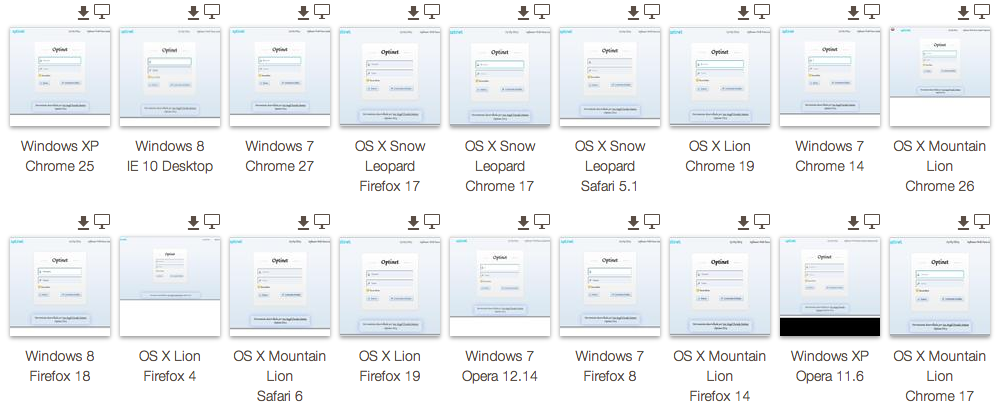
\includegraphics[scale=0.45]{browserstack.png}
  \caption{Compatibilidad en distintos navegadores}
  \label{a}
\end{figure}

\item \textbf{Mantenibilidad}:  Al utilizar Symfony2, la aplicación tiene una estructura de directorios predefinida que si el desarrollador la cumple, la aplicación será fácilmente mantenible ya que se sabrá donde se encuentran exactamente los archivos.

\item \textbf{Seguridad}: En la aplicación se ha tenido en cuenta los 10 fallos de seguridad más comunes en aplicaciones web indicados por la fundación OWASP en un documento.\footnote{\url{https://www.owasp.org/images/2/2d/OWASP_Top_10_-_2010_FINAL_(spanish).pdf}. \textit{OWAP - Los diez riesgos más importantes en aplicaciones web}}. 

\item \textbf{Fiabilidad}: A la aplicación desarrollada se le creó un plan de pruebas exhaustivo para que ésta funcionase sin cuelgues ni fallos.

\item \textbf{Interfaz de usuario}: Se utilizó la lista de los 25 puntos clave de usabilidad de UserEffect\footnote{\url{http://www.usereffect.com/download/checklist.pdf}. \textit{UserEffect}} comprobando que se cumplen todos los apartados.

\item \textbf{Rendimiento}: Se utilizaron las algunas herramientas online para probar el rendimiento de la aplicación obteniendo muy buenos resultados.
\begin{itemize}\renewcommand{\labelitemi}{$\diamond$}
\item \textbf{GTmetrix}\footnote{\url{http://gtmetrix.com}. \textit{GTmetrix}}:

\begin{figure}[!htb]
  \centering
    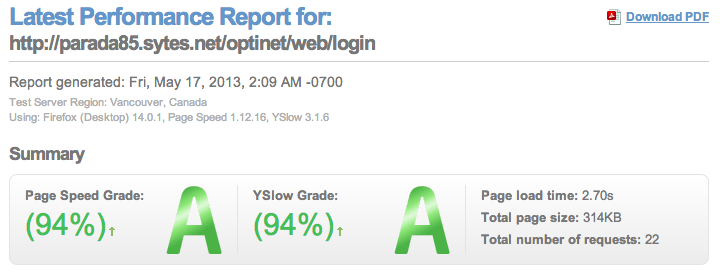
\includegraphics[scale=0.5]{ren.png}
  \caption{Rendimiento - GTmetrix   }
  \label{a}
\end{figure}

En esta web también podremos ver el historial de nuestra aplicación donde se puede apreciar como fuimos depurando la aplicación para obtener mejor puntuación y menor tiempo de respuesta:

\begin{figure}[!htb]
  \centering
    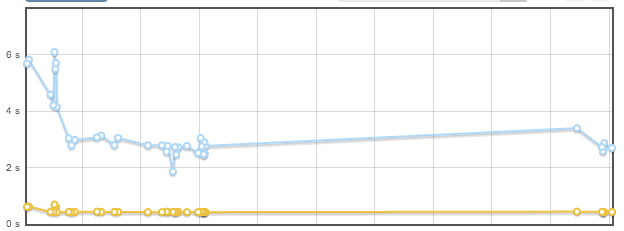
\includegraphics[scale=0.45]{ren1.png}
  \caption{Historial rendimiento 1 - GTmetrix   }
  \label{a}
\end{figure}

\newpage
\begin{figure}[!htb]
  \centering
    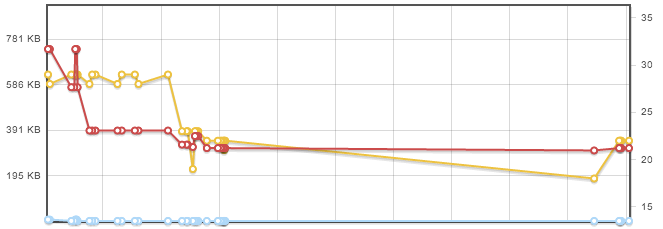
\includegraphics[scale=0.45]{ren2.png}
  \caption{Historial rendimiento 2 - GTmetrix   }
  \label{a}
\end{figure}

\begin{figure}[!htb]
  \centering
    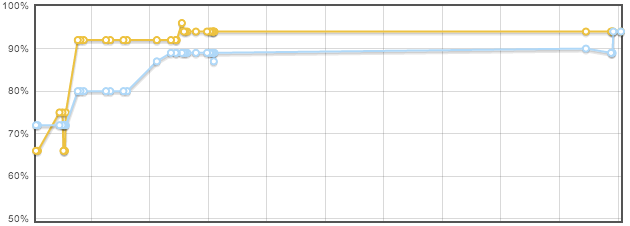
\includegraphics[scale=0.45]{ren3.png}
  \caption{Historial rendimiento 3 - GTmetrix   }
  \label{a}
\end{figure}


\newpage
\item \textbf{Pingdom Web Site Speed Test}\footnote{\url{http://tools.pingdom.com/fpt}. \textit{Pingdom}}: 

\begin{figure}[!htb]
  \centering
    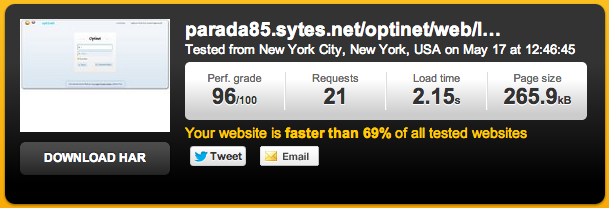
\includegraphics[scale=0.45]{renotro.png}
  \caption{Rendimiento - Pingdom}
  \label{a}
\end{figure}

\end{itemize}

También se probó el rendimiento de la aplicación con la ayuda de la biblioteca DoctrineFixturesBundle creando automáticamente multitud de clientes, proveedores y productos, comprobando que la aplicación tenía tiempos de espera cortos trabajando con numerosos datos.

\end{itemize}
\section {Pruebas de aceptación}

Una vez que se realizó la aplicación se realizaron pruebas de aceptación para comprobar que el sistema funcionaba correctamente. Este tipo de pruebas se realizaron con la ayuda del cliente.\\
La prueba de la aplicación se realizó atendiendo a dos tipos de personas, diferenciándose en los conocimientos informáticos:

\begin{itemize}
\item Personas con nivel alto de conocimientos informáticos:\\
Este grupo de personas que probaron la aplicación fueron compañeros de universidad que prestaron su tiempo para probar la aplicación utilizando sus conocimientos de codificación y sabiendo como funciona la aplicación por dentro.

\item Personas con nivel bajo de conocimientos informáticos:\\
Este grupo de personas son amigos que no dominan la informática pero que se defienden ya que usan los ordenadores para tareas diarias. También en este grupo de personas incluimos a los usuarios a los que va dirigida la aplicación.
\end{itemize}







